\documentclass{article}
\usepackage[utf8]{inputenc}

\title{MinaNarayananBioSu17}
\author{minaraya }
\date{May 2017}

\usepackage{natbib}
\usepackage{graphicx}

\begin{document}

\maketitle

\section{Introduction}
\subsection{Professional Bio}
\subsection{K12 Bio}
\subsubsection{Kindergarten}
\paragraph{Missing the Bus}
    
There is a theory which states that if ever anyone discovers exactly what the Universe is for and why it is here, it will instantly disappear and be replaced by something even more bizarre and inexplicable.
There is another theory which states that this has already happened.

In Kindergarten, I was 5 years old.

\begin{enumerate}
\item point
\end{enumerate}


\begin{itemize}
    \item Kindergarten - Fenner
    \item 1st Grade - Dobbins
\end{itemize}

\begin{figure}[b]
\centering
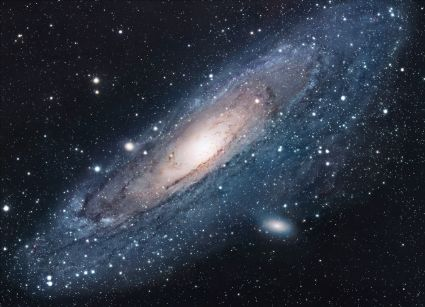
\includegraphics[scale=1.7]{universe.jpg}
\caption{The Universe}
\label{fig:universe}
\end{figure}

A picture of the universe is shown in Figure~\ref{fig:universe}.

\begin{figure}[h!]
\centering
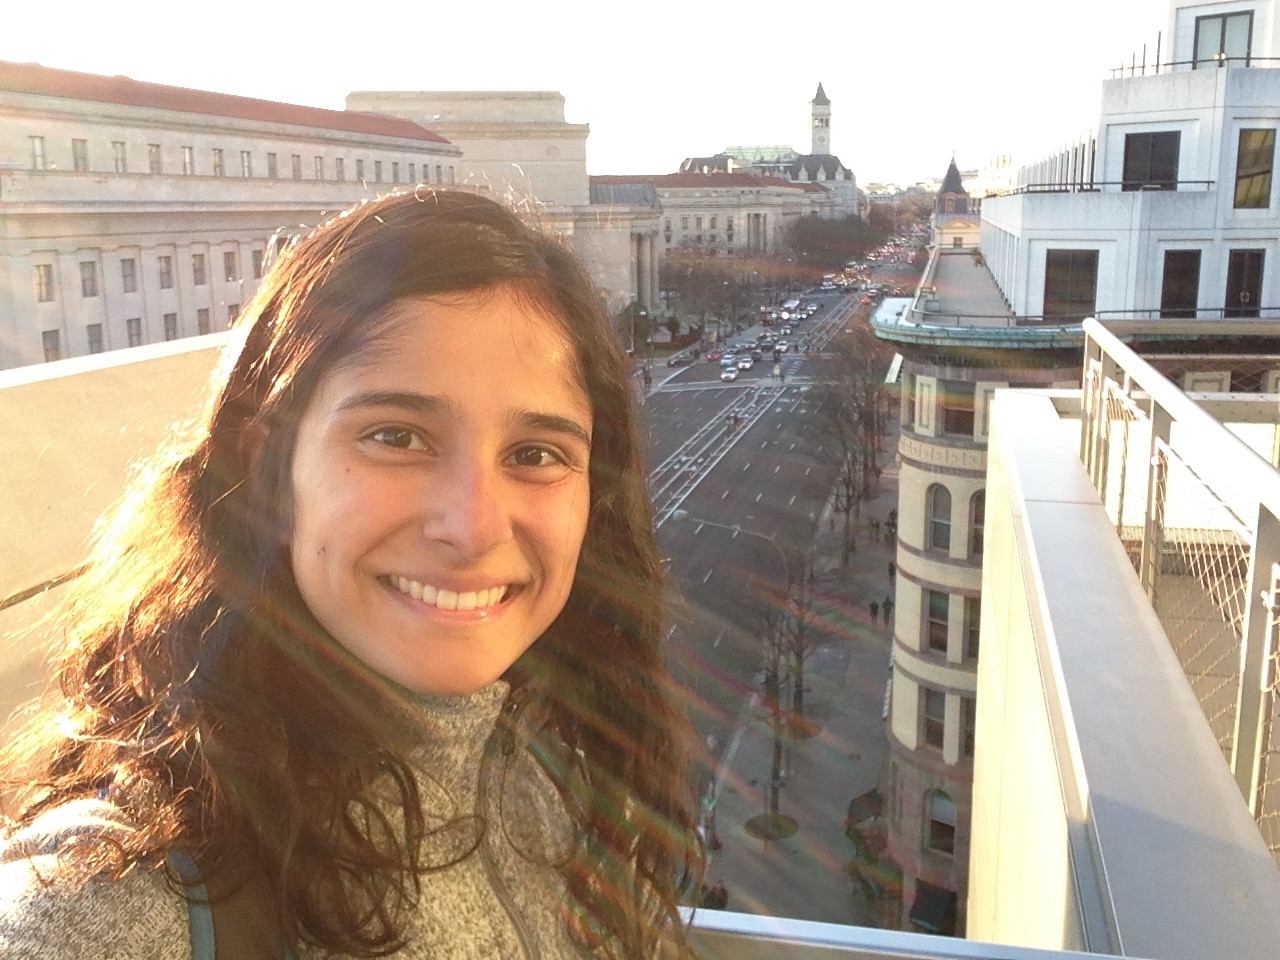
\includegraphics[scale=0.25]{Mina_N.JPG}
\caption{Mina Narayanan}
\label{fig:Mina_N}
\end{figure}

A picture of Mina Narayanan is shown in Figure~\ref{fig:Mina_N}. Mina has been involved in increasing diversity in computing since reading ???'s article~\cite{adams1995hitchhiker}.

\begin{table}
\begin{tabular}{lllcl}\hline{}
{\bf School} & {\bf Year} \\\hline
   Indian Pines & 2000-2003 \\
Dean Road Elementary School & 2003-2008 \\
Drake Middle School & 2008-2010\\
Auburn Junior High School & 2010-2012\\
Auburn High School & 2012-2015 \\
Auburn University & 2015-2017 \\\hline
\end{tabular}
\end{table}

\section{Conclusion}
``I always thought something was fundamentally wrong with the universe'' \citep{adams1995hitchhiker}

\bibliographystyle{apa}
\bibliography{references}
\end{document}
